
\documentclass[11pt,compress,t,notes=noshow]{beamer}

\usepackage[english]{babel}
\usepackage{dsfont}
\newcommand\bmmax{2}
\usepackage{bm}
\usepackage{bbm}
\usepackage{verbatim}
\usepackage{amsmath}
\usepackage{amsfonts}
\usepackage{csquotes}
\usepackage{multirow}
\usepackage{longtable}
\usepackage{enumerate}
\usepackage[absolute,overlay]{textpos}
\usepackage{psfrag}
\usepackage{algorithm}
\usepackage{algorithmicx}
\usepackage{algpseudocode}
\usepackage{eqnarray}
\usepackage{multimedia}
\usepackage{media9}
\usepackage{arydshln}
\usepackage{tabularx}
\usepackage{placeins}
\usepackage{tikz}
\usepackage{setspace}
\usepackage{wrapfig}
\usepackage{tcolorbox}
\usepackage[export]{adjustbox}
\usepackage{siunitx}
\usetikzlibrary{shapes,arrows,automata,positioning,calc}
\tikzset{
  %Define standard arrow tip
  >=stealth',
  %Define style for boxes
  punkt/.style={
    rectangle,
    rounded corners,
    draw=black, very thick,
    text width=6.5em,
    minimum height=2em,
    text centered},
  % Define arrow style
  pil/.style={
    ->,
    thick,
    shorten <=2pt,
    shorten >=2pt,}
}
\usepackage{subfig}

%new environments

\newenvironment{vbframe}  %frame with breaks and verbatim
{
 \begin{frame}[containsverbatim,allowframebreaks]
}
{
\end{frame}
}

\newenvironment{vframe}  %frame with verbatim without breaks (to avoid numbering one slided frames)
{
 \begin{frame}[containsverbatim]
}
{
\end{frame}
}

\newenvironment{blocki}[1]   % itemize block
{
 \begin{block}{#1}\begin{itemize}
}
{
\end{itemize}\end{block}
}

\newenvironment{fragileframe}[2]{  %fragile frame with framebreaks
\begin{frame}[allowframebreaks, fragile, environment = fragileframe]
\frametitle{#1}
#2}
{\end{frame}}


\newcommand{\myframe}[2]{  %short for frame with framebreaks
\begin{frame}[allowframebreaks]
\frametitle{#1}
#2
\end{frame}}

\newcommand{\remark}[1]{
  \textbf{Remark:} #1
}

%%%%%%%%%%%%%%%%%%%%%%%%%%%%%%%%%%%%%%%%%%%%%%%%%%%%%%%%%%%%%%%%%%%%%%%%%%%%%%%

% basic latex stuff
\newcommand{\pkg}[1]{{\fontseries{b}\selectfont #1}} %fontstyle for R packages
\newcommand{\lz}{\vspace{0.5cm}} %vertical space
\newcommand{\dlz}{\vspace{1cm}} %double vertical space
\newcommand{\oneliner}[1] % Oneliner for important statements
{\begin{block}{}\begin{center}\begin{Large}#1\end{Large}\end{center}\end{block}}


%\usetheme{lmu-lecture}
\usepackage{../style/lmu-lecture}

\let\code=\texttt
\let\proglang=\textsf

\setkeys{Gin}{width=0.9\textwidth}


\title{Deep Learning}
\author{Mina Rezaei}
\institute{Department of Statistics -- LMU Munich}
\date{Winter Semester 2021}

\setbeamertemplate{frametitle}{\expandafter\uppercase\expandafter\insertframetitle}

%\begin{document}
%\sloppy
%\end{document}

 
\input{../../latex-math/basic-math}
\input{../../latex-math/basic-ml}
\input{../../latex-math/ml-nn}

\begin{document}

\lecturechapter{9}{Specific AEs and Applications}
\lecture{Deeplearning}

\begin{frame}
\frametitle{Lecture outline}
\tableofcontents
\end{frame}

\section{Specific AEs and applications}
\begin{vbframe}{Convolutional autoencoder (ConvAE)}
  \begin{itemize}
    \item %n the last example, we have seen that autoencoder inputs are images. So, it makes sense to ask whether a convolutional architecture can work better than the autoencoder architectures discussed previously.
    For the image domain, using convolutions is advantageous. Can we also make use of them in AEs?     
    \item In a ConvAE, the encoder consists of convolutional layers. The decoder, on the other hand, consists of transpose convolution layers or simple upsampling operations.
   % \begin{itemize}
  %    \item Instead of convolving a filter mask with an image, to get a set of activations as in a CNN, we are trying to infer the activations that when convolved with the filter mask, would yield the image.
   % \end{itemize}
   % \item The original aim was to learn a hierarchy of features in an unsupervised manner. However, now its more commonly being used to invert the downsampling that takes place in a convolutional network and \enquote{expand} the image back to its original size.
  \end{itemize}
\framebreak
  \begin{figure}
    \centering
    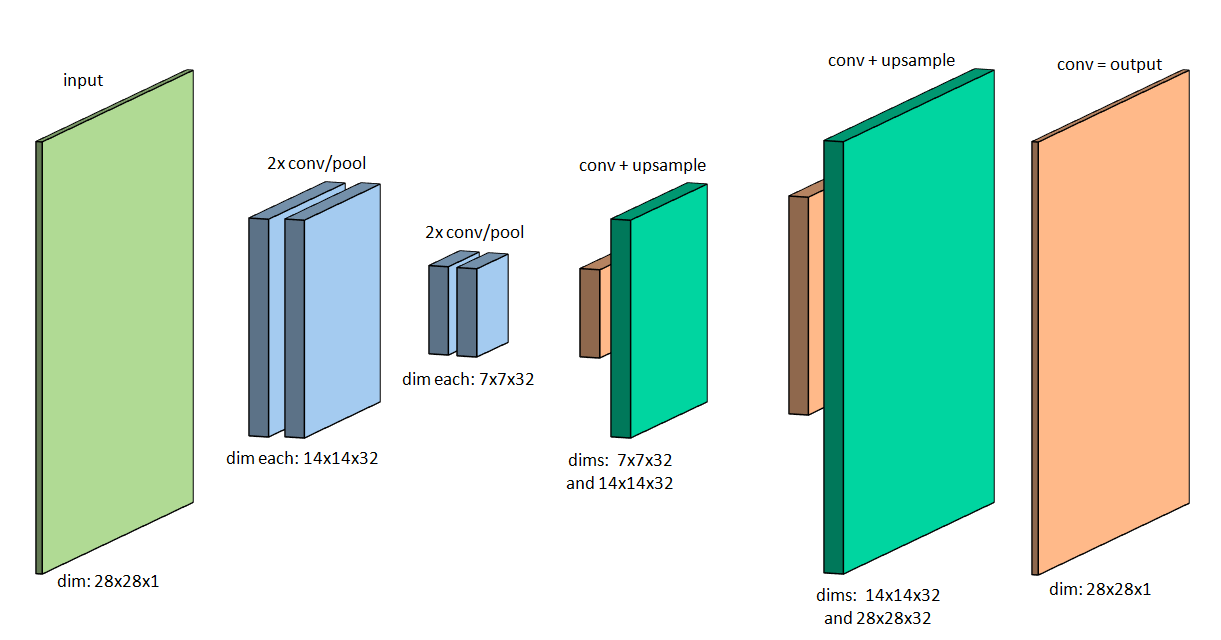
\includegraphics[width=11cm]{plots/convolutional_autoencoder3.png}
    \caption{Potential architecture of a convolutional autoencoder.}
  \end{figure}
  We now apply this architecture to denoise MNIST.
\framebreak
  \begin{figure}
    \centering
    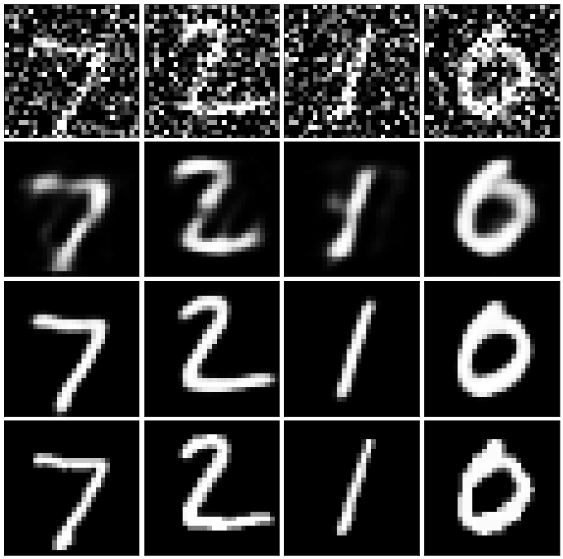
\includegraphics[width=6.3cm]{plots/convolutional_autoencoder2.png}
    \caption{Top row: noised data, second row: AE with $dim(\pmb{z}) = 32$ (roughly 50k params), third row: ConvAE (roughly 25k params), fourth row: ground truth.}
  \end{figure}
%\framebreak
%  Convolutional autoencoders may also be used for image segmentation:
%  \begin{figure}
%    \centering
%    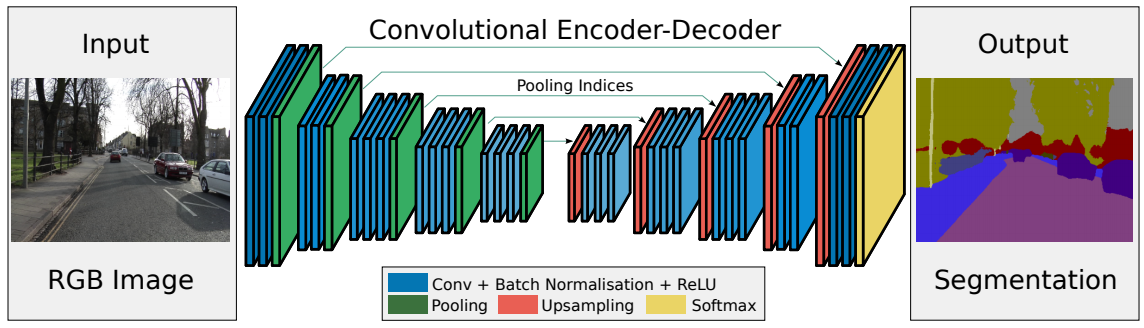
\includegraphics[width=11cm]{plots/convolutional_autoencoder.png}
%    \caption{SegNet: A Deep Convolutional Encoder-Decoder Architecture for Image Segmentation (Vijay Badrinarayanan et al. (2016))}
%  \end{figure}
\end{vbframe}
%%%%%%%%%%%%%%%%%%%%%%%%%%%%%%%%%%%%%%%%%%%%%%%%%%%%%%%%%%%%%%%%%%
%%%%%%%%%%%%%%%%%%%%%%%%%%%%%%%%%%%%%%%%%%%%%%%%%%%%%%%%%%%%%%%%%%
% \begin{vbframe}{AEs for unsupervised pretraining}
%   \begin{itemize}
%     \item Stacked AEs can be used for layer-wise unsupervised pretraining of deep neural networks.
%     \item This corresponds to subsequently training each layer as an AE.  
%     \item It aims  at yielding better weight initializations for the actual supervised training.
%     \item This usually eliminates the risk of vanishing gradients in feed forward nets.
%     \item It played an important role in the past before general techniques for stabilizing optimization were invented (e.g.~ReLUs, batch normalization, dropout, etc.)
%   \end{itemize}
% \end{vbframe}


\begin{vbframe}{Real-world Applications}

Today, autoencoders are still used for tasks such as: 
\begin{itemize}
\item  data de-noising,
\item  compression,
\item and dimensionality reduction for the purpose of visualization.
\end{itemize}

\framebreak 
  \textbf{Medical image denoising} using convolutional denoising autoencoders
  \begin{figure}
    \centering
    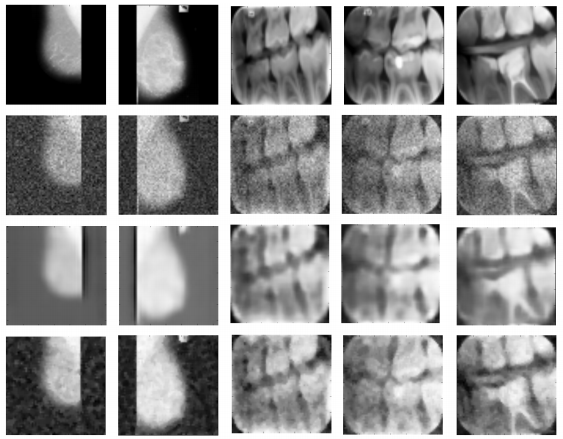
\includegraphics[width=6.5cm]{plots/denoising_autoencoder_application.png}
    \caption{Top row : real image, second row   : noisy version, third row : results of a (convolutional) denoising autoencoder and fourth row : results of a median filter (Lovedeep Gondara (2016))}
  \end{figure}
  
  \framebreak
  AE-based \textbf{image compression}.
  \begin{figure}
    \centering
    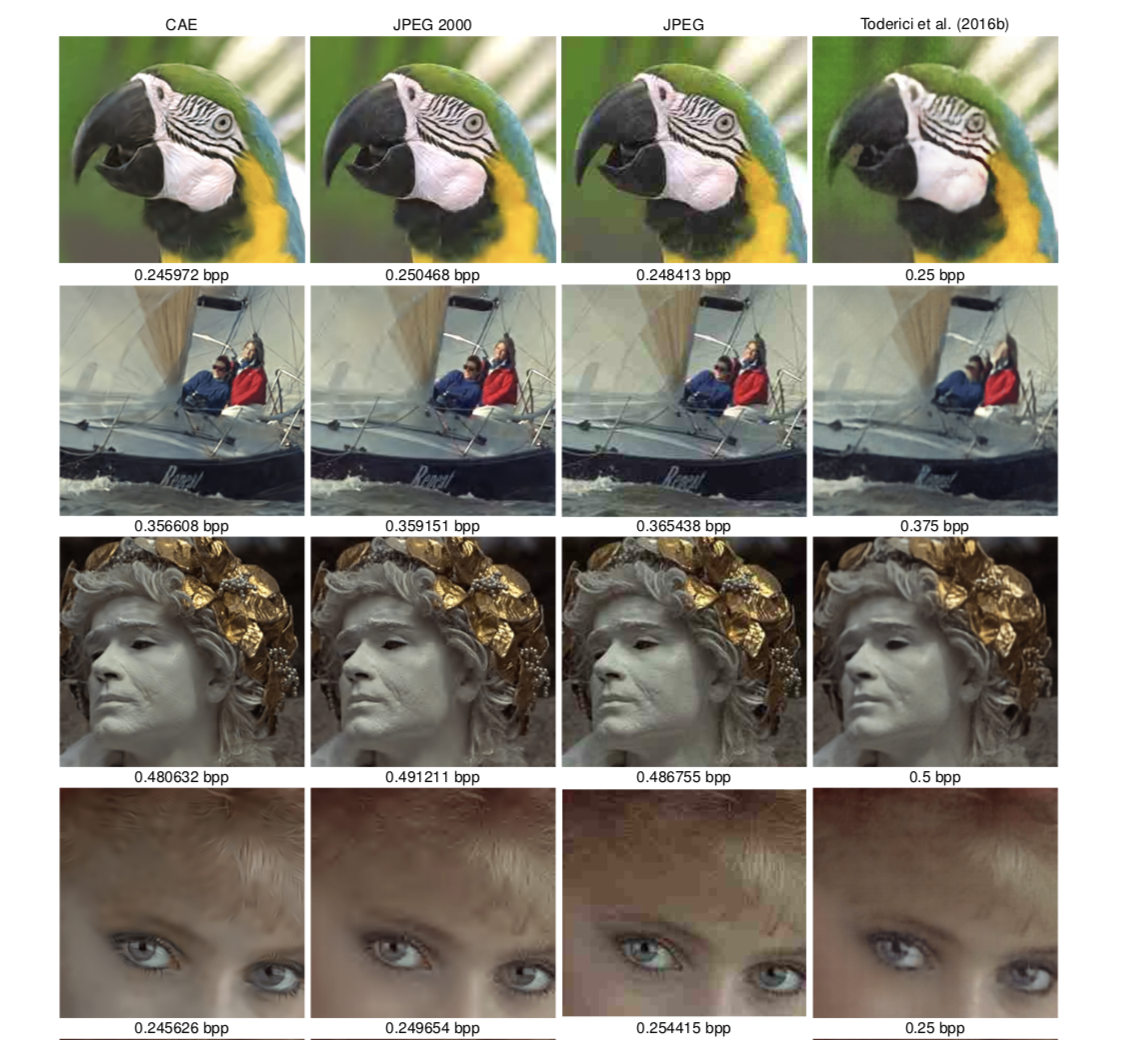
\includegraphics[width=6.5cm]{plots/image-compression.png}
    \caption{from Theis et al. }
    \end{figure}
  
  
\end{vbframe}


\endlecture
\end{document}